\section{Cardinal}
\label{s:cardinal}

MOOSE was initially developed for solving fully coupled systems of partial
differential equations (PDEs) using fully implicit timestepping. To utilize
MOOSE, developers create small C++ objects representing their PDEs, boundary
conditions, initial conditions, and so forth. MOOSE then coordinates PETSc and
libMesh \cite{kirk2006libmesh} to perform a Newton solve over all of the
physics to find the solution to the multiphysics problem. While this is still
the primary way to use MOOSE, the library has also gained capability for
loosely coupled solves, Picard iteration, and even coupling to external
applications (such as OpenMC and Nek5000).  In this section we discuss the
MultiApp features of MOOSE used in Cardinal.  A new MOOSE-based application was
created \cite{cardinal}  that compiles all of the codes into one executable.
For the previous study, that code was named Cardinal and combined BISON,
OpenMC, and Nek5000 to achieve high-fidelity simulation of FHR reactors.

\subsection{MOOSE Coupling Capability}

The MultiApp system within MOOSE allows for arbitrary-depth, hierarchical execution of applications in parallel \cite{gaston2015physics}. As shown in Figure \ref{f:moose1}, a MultiApp solve will always have a master application. Underneath that master application can be an arbitrary number of MultiApp objects. The MultiApp objects are containers of instances of applications and can have many instances of that application. As an example, the master application might be a neutron transport simulator for light-water reactors and have one MultiApp representing the fuel rods with that MultiApp having thousands of instances of a fuel performance simulation tool, one for each fuel rod. Each subapp itself can have any number of MultiApps, leading to an arbitrarily deep tree of applications. These application instances are spread out in parallel, and all subapps within an individual MultiApp are executed simultaneously (given enough computing resources).

\begin{figure}[!h]
\centering
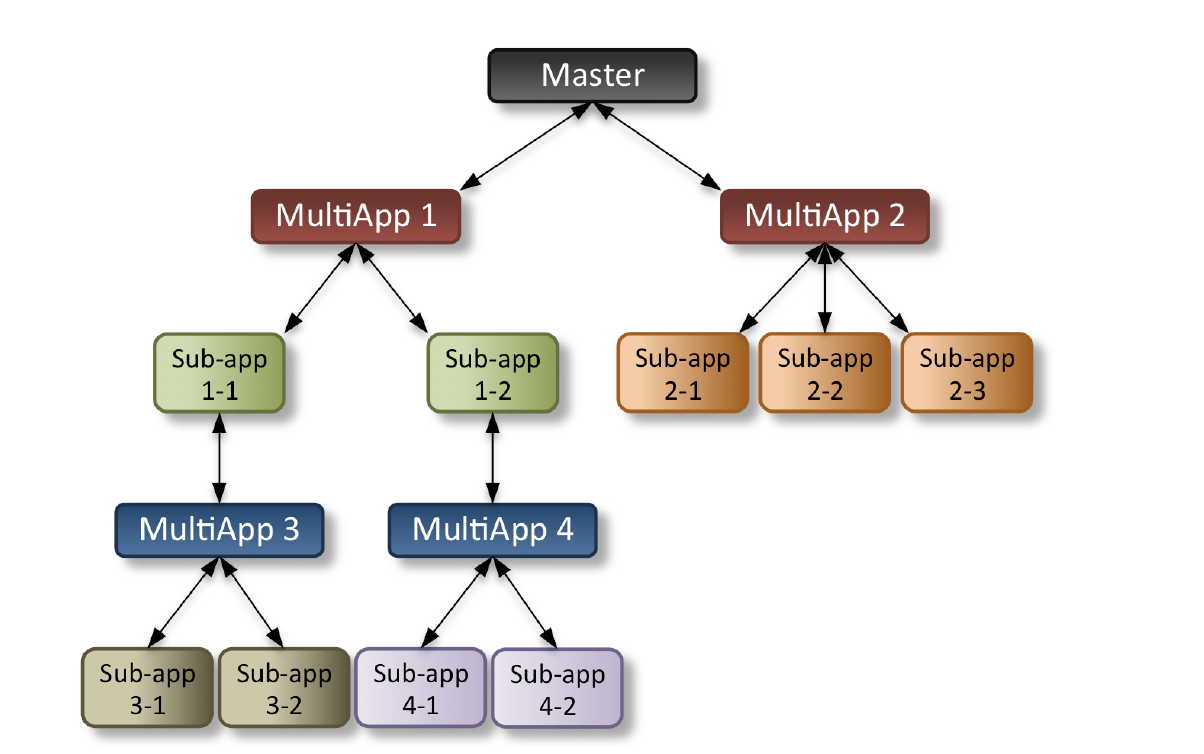
\includegraphics[clip=true,width=0.9\textwidth]{Figures/moose1}
\caption{MultiApp structure.}
\label{f:moose1}
\end{figure}


Critical to Cardinal is that a MultiApp can hold non-MOOSE-based (``external'')
applications. This is possible using the Moose-Wrapped-App (MWA) interfaces. By
creating a few objects that wrap an external app and present it to MOOSE as a
MOOSE-based application, that external application can then be placed into any
point in the hierarchy. For the current effort, OpenMC and Nek5000 were wrapped
in the MWA interfaces, allowing them to participate in a MultiApp solve. For
each application the following interfaces were developed:

\begin{itemize}
    \item \textit{ExternalApp}: Derives from MooseAppBase and is the basic wrapper to the code the MultiApp
    system needs.
    \item \textit{ExternalProblem}: Derives from Problem to implement solve(), which calls the external code and creates data fields.
    \item \textit{ExternalMesh}: Derives from MooseMesh to create a mesh that is compatible with the external app.
\end{itemize}
While MultiApps create trees of executing applications, transfers are needed to move data between them. Transfers move data only vertically, up and down the hierarchy of applications. Many different types of transfers exist, including interpolation projection, evaluation, data copy, post-processor transfer, and scalar variable transfer.
%\begin{itemize}
%  \item Interpolation
%  \item Projection
% \item Evaluation
%  \item Data-copy
%  \item Postprocessor transfer
%  \item Scalar Variable transfer
%\end{itemize}
Consistent data transfers between dissimilar applications pose challenges for massively parallel code execution.  The MWA system utilizes an ExternalMesh that is created to be compatible with the third-party application to address this issue. Fields/values can then be easily moved to the ExternalProblem (fields) that uses the ExternalMesh. Built-in MOOSE transfers can communicate those values with any other MOOSE/non-MOOSE application in the MultiApp hierarchy. A schematic describing the solution transfer is shown in Figure~\ref{f:moose2}.

\begin{figure}[!h]
\centering
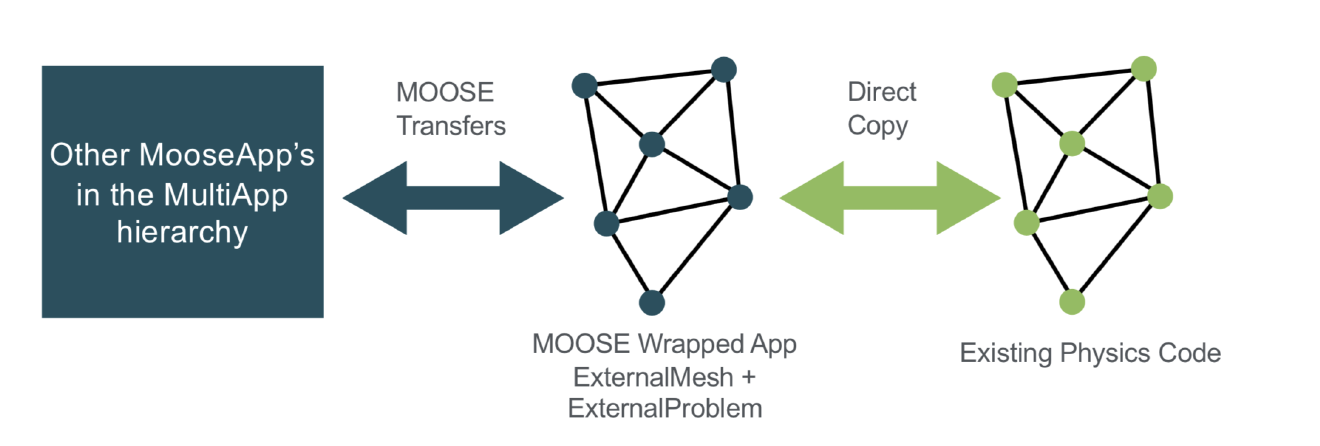
\includegraphics[clip=true,width=0.9\textwidth]{Figures/moose2}
\caption{Solution transfer.}
\label{f:moose2}
\end{figure}

MOOSE also provides the ability to solve for coupled physics in three primary ways:
\begin{itemize}
\item Loosely coupled: each physics solved with a separate linear/nonlinear solve. Data exchange once per
timestep (typically).
\item Tightly coupled / Picard: each physics solved with a separate linear/nonlinear solve. Data is exchanged, and physics re-solved until convergence.
\item Fully coupled: all physics solved for in one linear/nonlinear solve.
\end{itemize}
These three options are depicted in Figure~\ref{f:moose3}. The top coupling represents a one-way loose coupling where, in each timestep, one physics is solved, and the solution is passed to the next physics solver. The other physics is then solved, and time marches forward. The second coupling utilizes Picard iteration to converge the two physics within each timestep. The final coupling method, the one originally utilized by MOOSE, is full coupling: all PDEs within the system are solved simultaneously, resulting in a completely converged solution within one solve. While fully coupled simulation has many advantages when physics are interdependent, it can be
overly burdensome for more loosely coupled physical systems. Therefore, utilization of the MultiApp and transfer systems for loose coupling and Picard iteration can be useful for multiscale solves, solves involving multiple timescales, and solves utilizing external applications. The Cardinal application developed for lower length scale simulation of FHRs utilizes MultiApps for just this purpose: coupling Nek5000, OpenMC, and BISON.

\begin{figure}[!h]
\centering
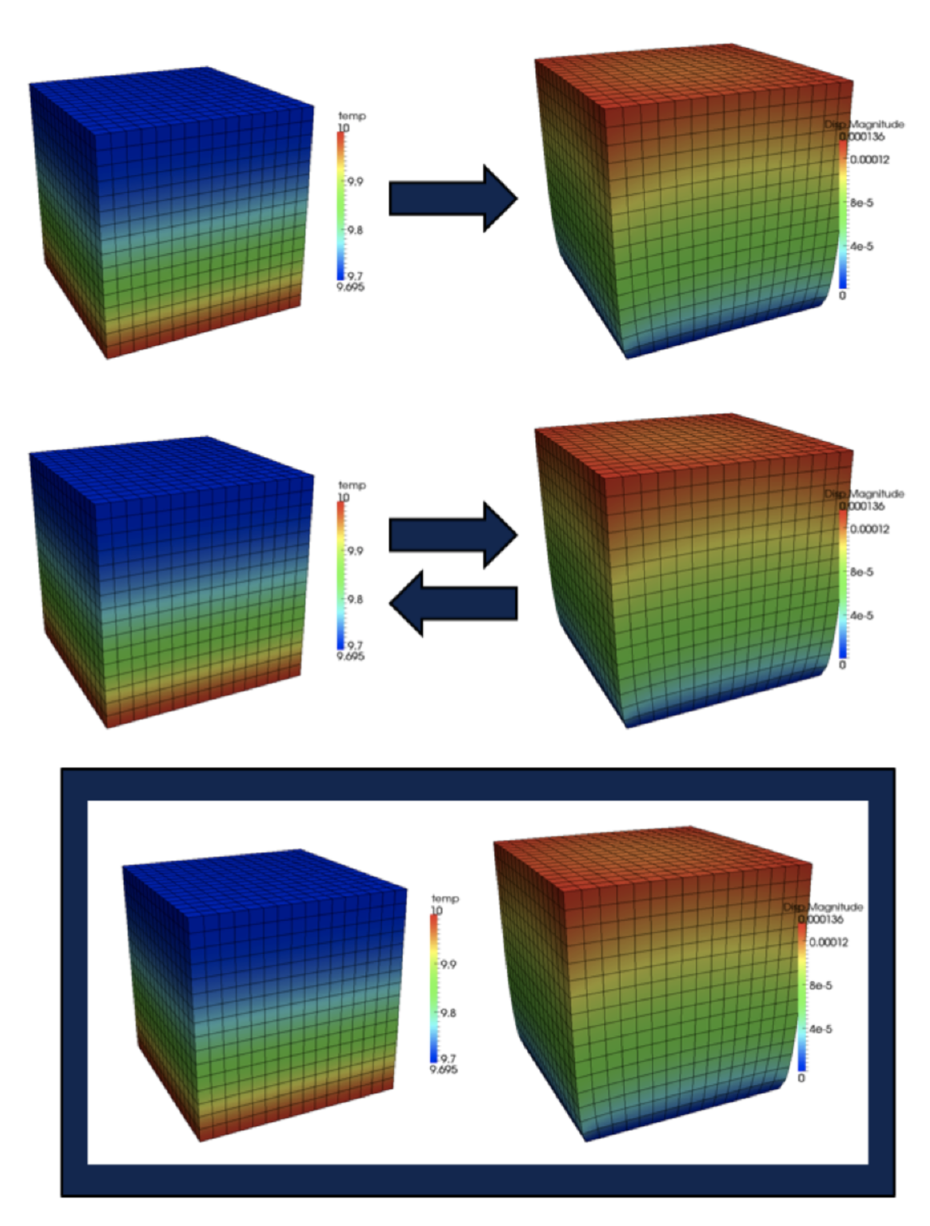
\includegraphics[clip=true,width=0.9\textwidth]{Figures/moose3}
\caption{MOOSE coupling strategies. Top: loose, Middle: Picard, Bottom: full.}
\label{f:moose3}
\end{figure}

\subsection{Design of Cardinal}
\label{ss:c1}

Cardinal utilizes the MOOSE MultiApp capability to place each of the applications to be coupled within a hierarchical tree-based structure, as shown in Figure~\ref{f:cardinal}. This structure was chosen based on how tightly coupled the physics are. BISON and Nek5000 form one branch because of the instantaneous feedback between the conjugate heat transfer and the pebble temperature. The Nek5000 solution provides the temperature boundary condition on each pebble exterior, while BISON returns the heat flux at each point around the pebble to Nek5000. Another benefit of having BISON and Nek5000 on their own branch is the way it impacts timestepping. Within the MultiApp setup shown in Figure \ref{f:cardinal}, the branch containing BISON and Nek5000 can take many small timesteps and even iterate between BISON and Nek5000 within a timestep without needing to re-solve OpenMC. This can significantly reduce the time to solution of the application. OpenMC is then separate from the other two. It receives fuel/pebble temperatures from BISON and returns a heat source that is transferred down to BISON. OpenMC is currently solving for steady-state neutronics and can take larger timesteps compared with BISON and Nek5000 (which are both performing transient heat conduction and CFD solves, respectively). The flexibility of the MOOSE MultiApp system allows for just such a setup.

\begin{figure}[!h]
\centering
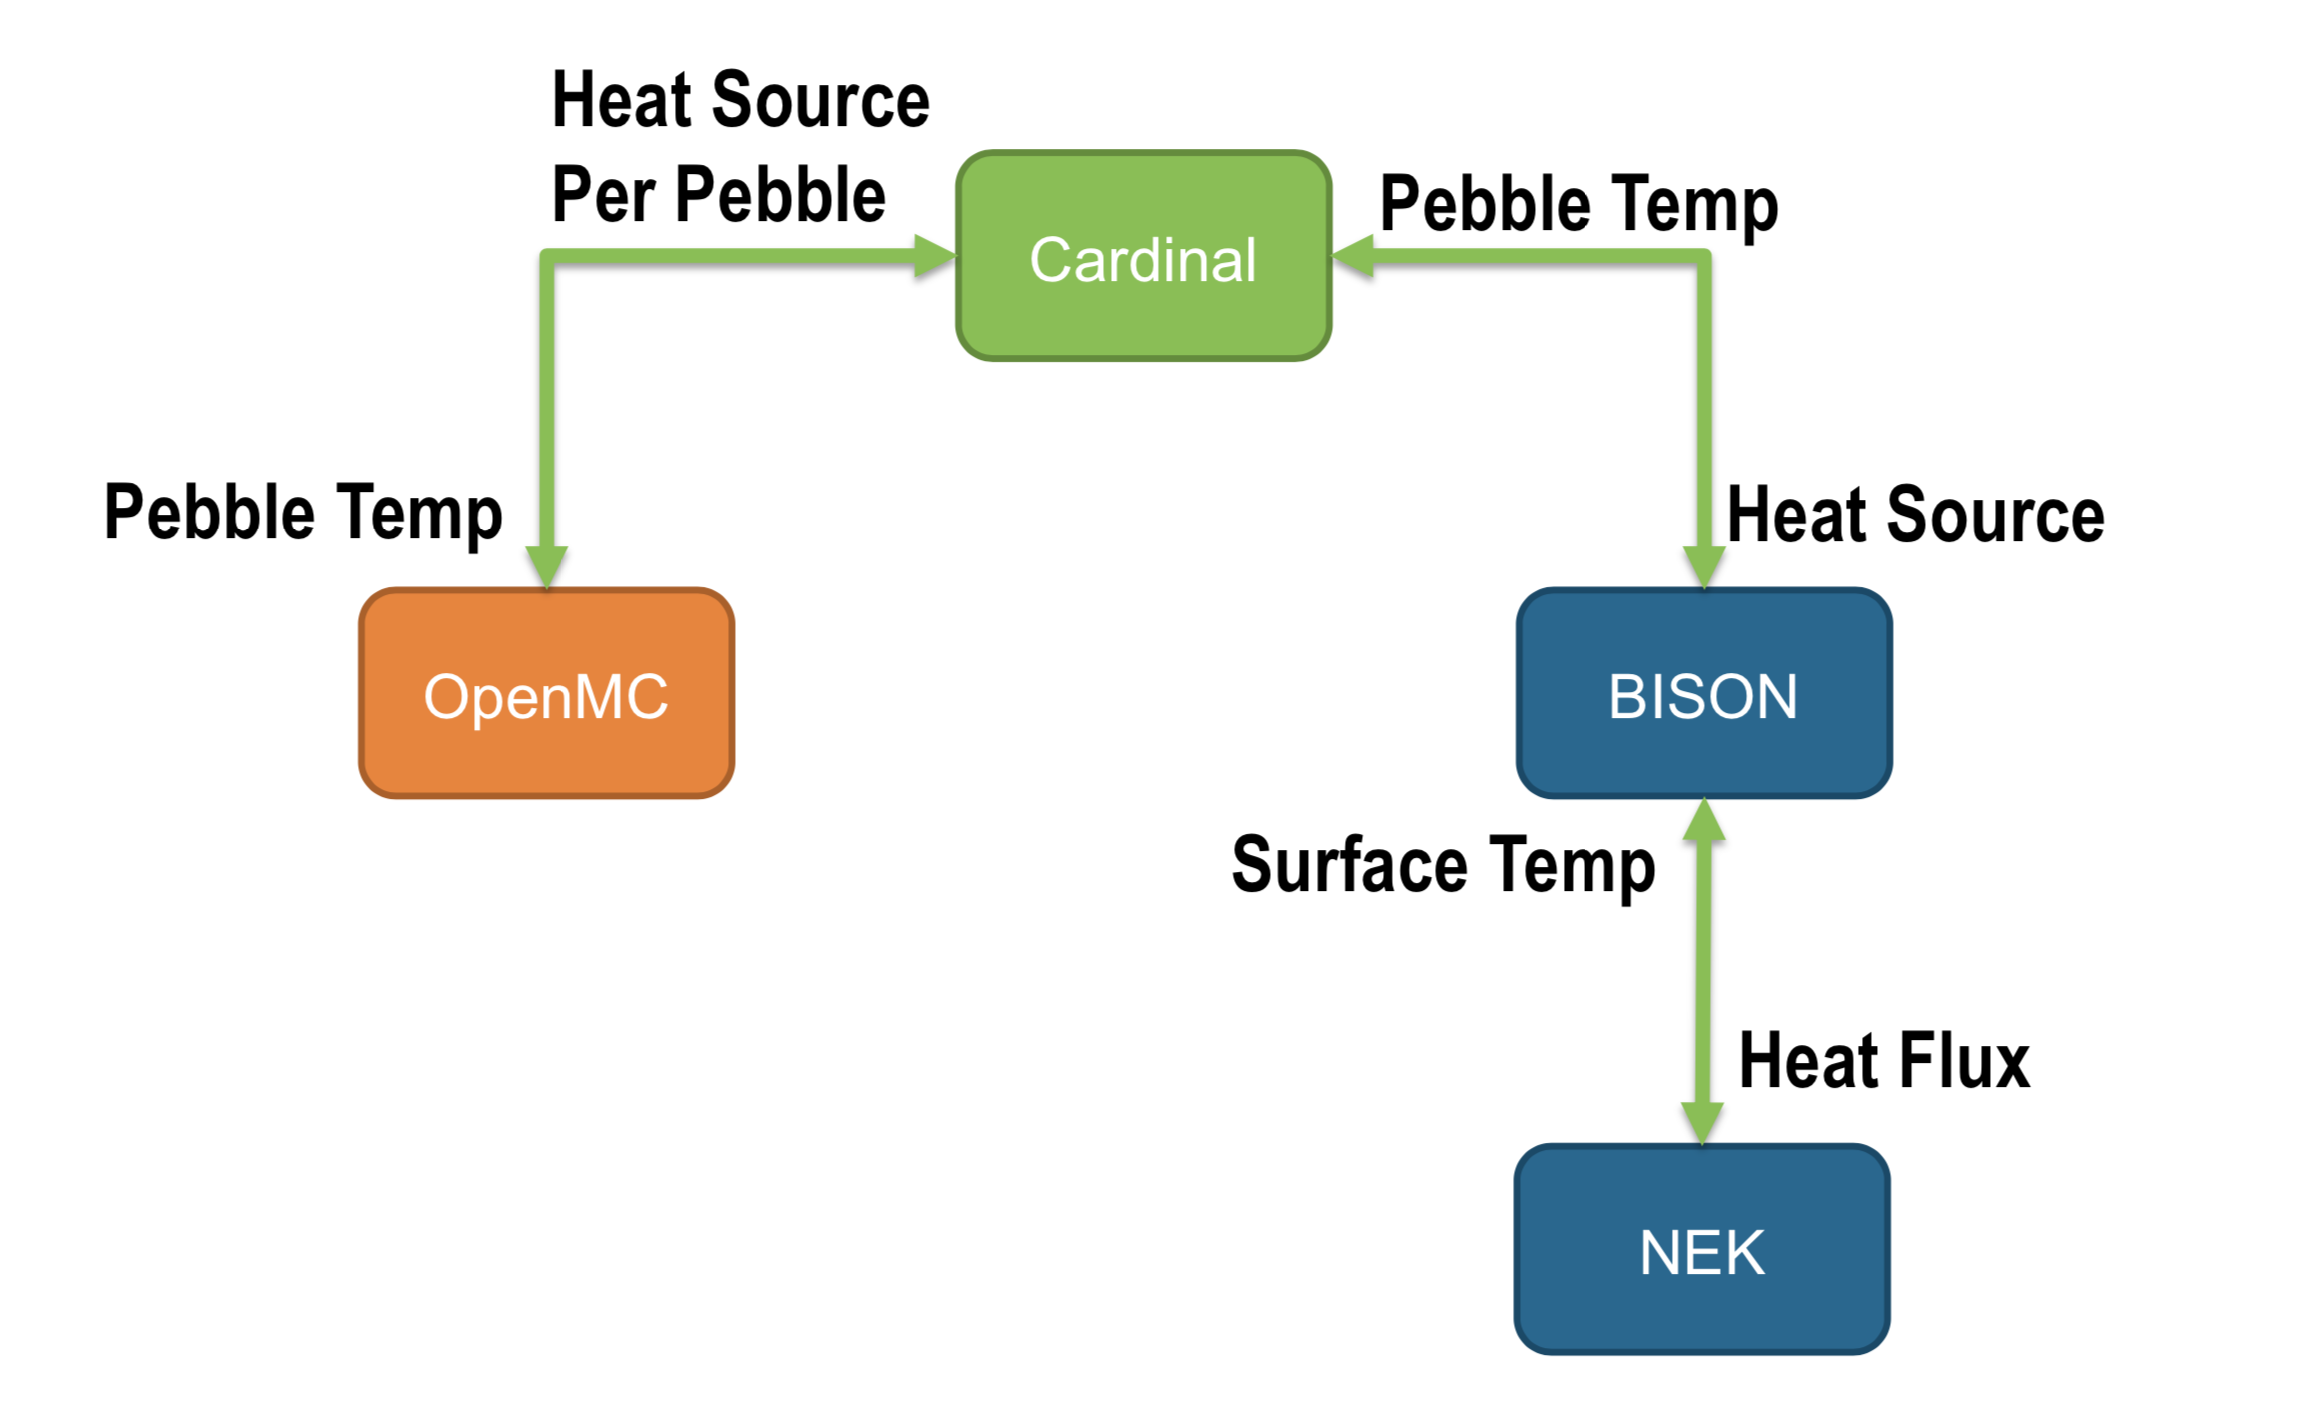
\includegraphics[clip=true,width=0.9\textwidth]{Figures/cardinal}
\caption{Diagram showing the design of Cardinal.}
\label{f:cardinal}
\end{figure}

\subsubsection{Build System}
\label{ss:c2}

In any multiphysics coupling project with many dependent libraries, ensuring consistent compilation and linking can be a challenge. Throughout Cardinal, we rely on PETSc to detect system-dependent configuration information and install as many third-party libraries as possible (Figure~\ref{f:build}). BISON, MOOSE, and libMesh already rely on PETSc, and they are built as usual. For standalone OpenMC and
Nek5000, PETSc is not a dependency; but in Cardinal, OpenMC and Nek5000 use PETSc for two purposes:
\begin{itemize}
\item PETSc is built on top of HDF5 and BLAS/LAPACK, which are also dependencies of OpenMC and Nek5000, respectively.
\item The configuration info discovered by PETSc is passed to the build systems of OpenMC and Nek5000.
\end{itemize}
This is done through header files that PETSc generates specifically for this purpose. Hence, after installing PETSc and libMesh, Cardinal can be built in one step.
%% NOTE: to math the diagram, not introducing NekRS yet, while still true statement.
%%We have added a branch of the repository that compiles NekRS instead of Nek5000. The build system also allows Cardinal to run on the Summit supercomputer at ORNL.
The build system also allows Cardinal to run on the Summit supercomputer at ORNL.
\begin{figure}[!h]
\centering
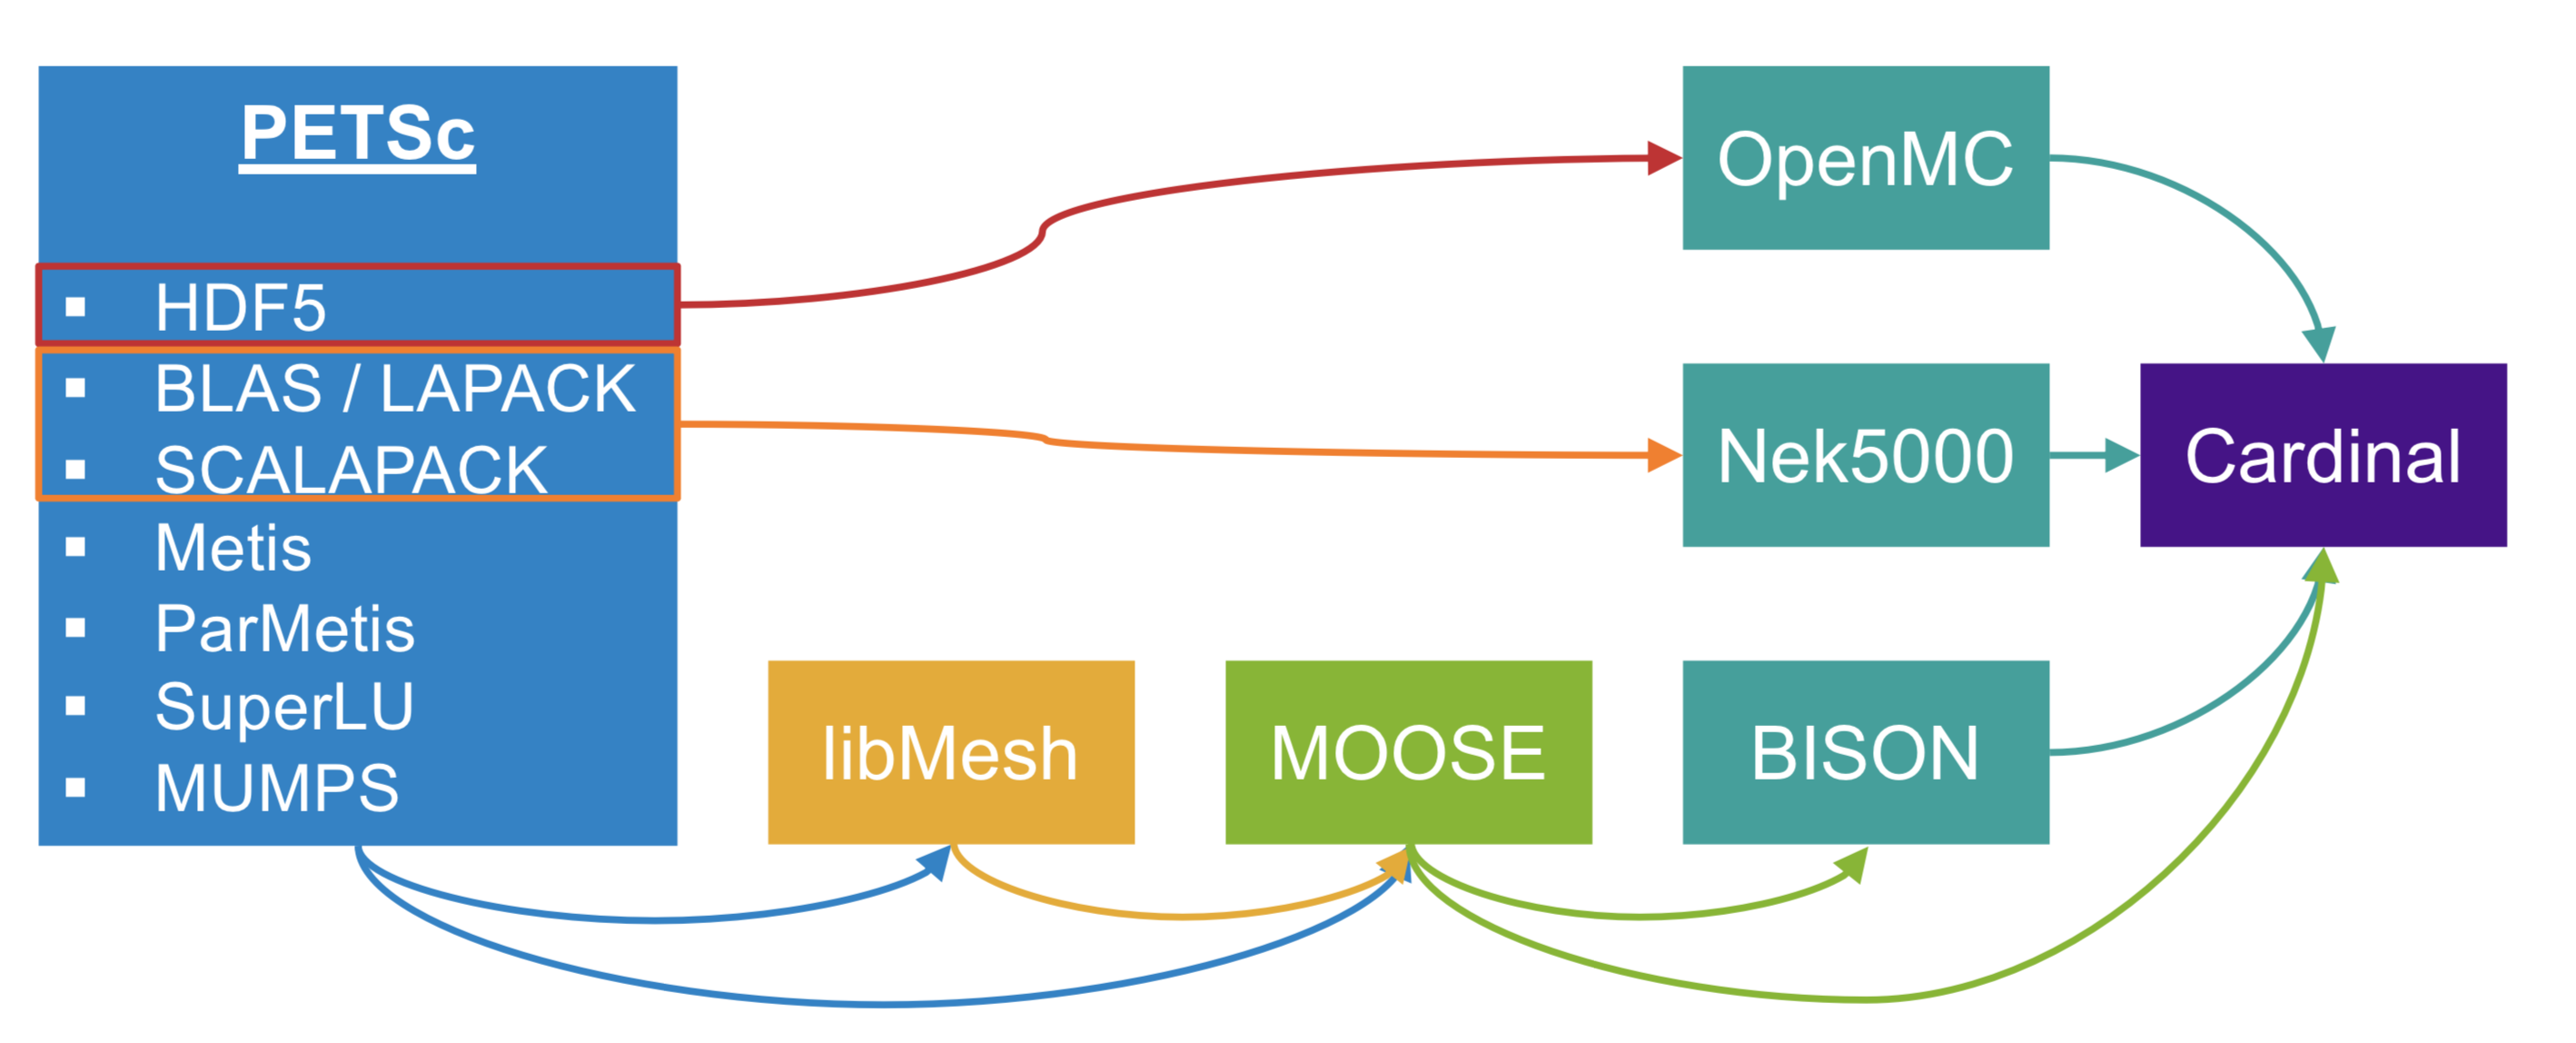
\includegraphics[clip=true,width=0.9\textwidth]{Figures/build}
\caption{Diagram describing the build system of Cardinal.}
\label{f:build}
\end{figure}

\subsubsection{Nek5000/NekRS and API}

Nek5000 \cite{fischer2015nek5000} is an open-source simulation software package
that delivers highly accurate solutions for a wide range of scientific
applications, including fluid flow, thermal convection, combustion, and
magnetohydrodynamics. It features state-of-the-art, scalable high-order
algorithms that are fast and efficient on platforms ranging from laptops to the
DOE leadership computing facilities.

Nek5000 is based on the spectral element method \cite{patera1984} in which  the
domain is decomposed globally into smaller domains (elements), which are
assumed to be curvilinear hexahedra (brick meshes) conforming to the domain
boundaries. Locally, functions within each element are expanded in high-order
(typically $N=4$--12) tensor-product polynomials.  The pressure can be solved
at the same polynomial order as the velocity $N$ ($P_{N} - P_{N}$ formulation)
or at lower order $N-2$ ($P_{N} - P_{N-2}$ formulation).  Temporal
discretization is based on a high-order splitting that is third-order accurate
in time and reduces the coupled velocity-pressure Stokes problem to four
independent solves per timestep: one for each velocity component and one for
the pressure. The velocity problems are diagonally dominant and thus easily
solved by using Jacobi preconditioned conjugate gradient iteration. Two
timestepping schemes, both up to third order, are available: semi-implicit
BDF-extrapolation or subcycle-based characteristics. The characteristics
scheme permits relatively large timesteps corresponding to CFL numbers
of 4 or more \cite{patel19}. The pressure substep requires a Poisson solve
at each step, performed through multigrid-preconditioned GMRES iteration
coupled with temporal projection to find an optimal initial guess.
Particularly important components of Nek5000 are its scalable coarse-grid
solvers that are central to parallel performance. For both weak and
strong scaling, using algebraic multigrid for the coarse-grid solve is
essential above 250,000 elements. Nek5000 employs a pure MPI parallel
implementation.  An extensive discussion of the scalability of Nek5000 is
provided in \cite{fischer15,fischer20a}.

We note that Nek5000 relies on hexahedral conformal meshes, which are generally
more challenging to construct than meshes with tetrahedral elements.  We have
developed a \textit{tet-to-hex} technique that enables the use of Nek5000 on
complex geometries and that produces remarkably well-conditioned meshes
\cite{yuan2020spectral}.  Our early trials for the pebble bed are based on this
approach.  To scale to very large pebble counts, however, we are developing a
tailored approach to the generation of all-hex meshes in the pebble void regions
that is base on a a tessellation of the Voronoi cells defined by the pebble
centers.  The Voronoi cells are generated using matlab or other off-the-shelf
software.  In the domain interior, each facet is associated with two spheres.
The facet is tessellated into a few quadrilaterals, the images of which are
then projected onto the spheres resulting in a valid baseline all-hex mesh.
Facets on the domain boundary are generated by having image elements reflected
through the boundary to the domain exterior.  These are similarly partitioned
and projected onto the single interior sphere that they face.  The elements
swept out by the projection process are partitioned radially (typically into
three elements in the radial direction) and the overall mesh is smoothed using
the algorithms presented in \cite{mittal19a}.  Refinements of the algorithm
include deletion (collapse) of short edges in the Voronoi cells and insertion
of points on long edges in order to produce a more uniform mesh throughout the
domain.  The Voronoi-based approach leads to a six-fold reduction in element
count (thus enabling the use of higher polynomial order) and significant
reduction in the CFL for a given timestep size compared to the more general
tet-to-hex strategy.  We demonstrate the results for this approach for
pebble-bed examples in later sections.

Nek5000 couples to MOOSE in a simple way:
\begin{itemize}
 \item A point cloud with the GLL points corresponding to the surface mesh
      (corresponding to either $N = 2$ or $N = 1$) is defined. The points are
      used by MOOSE to define a mapping.
 \item A set of routines is then defined for solution transfer. The temperature
      is extracted on the Nek5000 mesh and loaded onto the points cloud in MOOSE.
 \item The flux data is loaded from the points cloud and used to reconstruct
      an arbitrary order $N$ surface field for the heat flux.
 \item A set of routines for timestepping is defined.
\end{itemize}
We note that even with a relatively large problem like the demo problem
discussed in this manuscript, the solution transfer's memory footprint and
computational cost are not significant compared with the physics solves.

Cardinal also interfaces with NekRS, a new GPU-oriented version of Nek5000
that is also capable of running on CPUs. It represents a significant redesign
of the code.  While written in C++, NekRS is able to link to Nek5000 to
leverage its extensive pre- and postprocessing utilities.  NekRS has been
built primarily under the auspices of the DOE Exascale Computing Project. It
realizes high throughput on advanced GPU nodes and demonstrates excellent
scalability.  Details of NekRS performance for nuclear applications are
provided in recent publications \cite{merzari2020toward}. The Cardinal API of
NekRS heavily uses the Cardinal API of Nek5000 and yields identical results.

All pebble bed simulations performed here use either LES, using an explicit
filter \cite{fischer2001filter}, or direct numerical simulation (DNS). The CFD
resolution requirements are thus significant---about 150,000 points per pebble.
The rapid convergence of the high-order discretizations in Nek5000 and NekRS
and their high performance on the DOE's leadership computing facilities makes
them ideally suited for this set of simulations.

\subsubsection{OpenMC and API}

OpenMC \cite{romano2015openmc} is a general-purpose Monte Carlo particle transport simulation code focused on coupled neutron--photon calculations. It is
capable of simulating 3D models based on constructive solid geometry with second-order surfaces or CAD geometries. OpenMC
supports either continuous-energy or multigroup transport. The continuous-energy particle interaction data
is based on a native HDF5 format that can be generated from ACE files used by the MCNP and Serpent
Monte Carlo codes. Additionally, OpenMC can use multipole cross-section data for temperature feedback
calculations (as in Cardinal).

For Cardinal, we use the C/C++ API of OpenMC to start and stop the simulation at various levels (including the overall
simulation and individual batches) and for accessing underlying data structures (such as cell, material, and
tally data) during online coupling.

Like several other MC transport simulators (such as MCNP), OpenMC uses constructive solid geometry (CSG) to build models in Euclidean space.
Volumes called half-spaces are bounded by quadratic surfaces, which are defined by parameterized equations, not gridpoints. A given surface defines a positive and negative half-space, and Boolean combinations (intersections, unions, and differences) of these half-spaces can form arbitrarily complex volumes. In OpenMC, a Boolean combination of arbitrarily many half-spaces describes a volume called a cell. Moreover, in OpenMC, each cell contains one or more materials; each material in turn contains information about nuclide identities, nuclide atom densities, and overall material density. Each cell also contains temperature information; note that temperature information is not associated with the material itself.

Previous efforts have attempted to couple OpenMC to MOOSE for LWR applications \cite{ellis2017preliminary}.
However, the current effort takes a new approach. In particular, we have implemented two options:
\begin{itemize}
    \item \textbf{A cell-based API.}.  We leverage MOOSE Wrapped-Apps features to develop a specialized interface for the PBR problem. To transfer temperature from BISON to OpenMC, we must update the temperature of an OpenMC cell, which updates the temperature of each material in the cell. Heat sources are also tallied on each pebble and transferred to BISON.
    \item \textbf{A mesh-tally API}.
\end{itemize}

In the following, we discuss in more detail the mesh-tally API. In order to capture heat generation in the OpenMC simulation, a tally scoring total recoverable fission energy per source particle is applied to each pebble's outer cell in the bed. These tallies are created at runtime during the problem setup by using a list of pebble centers to locate the uppermost cell in the CSG geometry hierarchy containing that point.

As summarized in \autoref{eq:heat_source_normalization}, the energy deposition for each pebble, $\hat{q}_{i}$, is normalized by the total energy deposition in the bed.  This value is then multiplied by the total thermal power of the reactor, $Q$, to obtain an average heat generation rate for each pebble, $q_i$, and divided by the volume of each pebble, $V_p$, to obtain a volumetric heat generation rate, $q'''_i$.

\begin{equation}
    \label{eq:heat_source_normalization}
    q'''_i = \frac{Q q_i}{V_{p}\sum_{i}{\hat{q_i}}} = \frac{[W][J/source]}{[cm^{3}] [J/source]} = \frac{[W]}{[cm^{3}]}
\end{equation}

This results in a single average heating value for the entire pebble. Before being transferred to the MOOSE mesh, these values are normalized by the total heat.

For improved spatial resolution of heat generation in the pebble bed, unstructured mesh tallies have been implemented in OpenMC. \autoref{fig:pebble_umesh} provides an example of this capability applied to a single pebble. The unstructured mesh representation relies on a LibMesh mesh instance and currently conforms to the OpenMC tally data model that separates the mesh structured from the tally data itself. The separation of this information allows the unstructured mesh to be applied in a mesh filter object that is agnostic to the underlying mesh type. The mesh filter can then be combined with other specified filters, scores, and nuclides in a tally and can be used in one or more tally definitions. Calls into the LibMesh library from OpenMC are agnostic to the type of elements used, so meshes can be formed by using any element type supported by LibMesh.

\begin{figure}
    \centering
    \raisebox{-0.5\height}{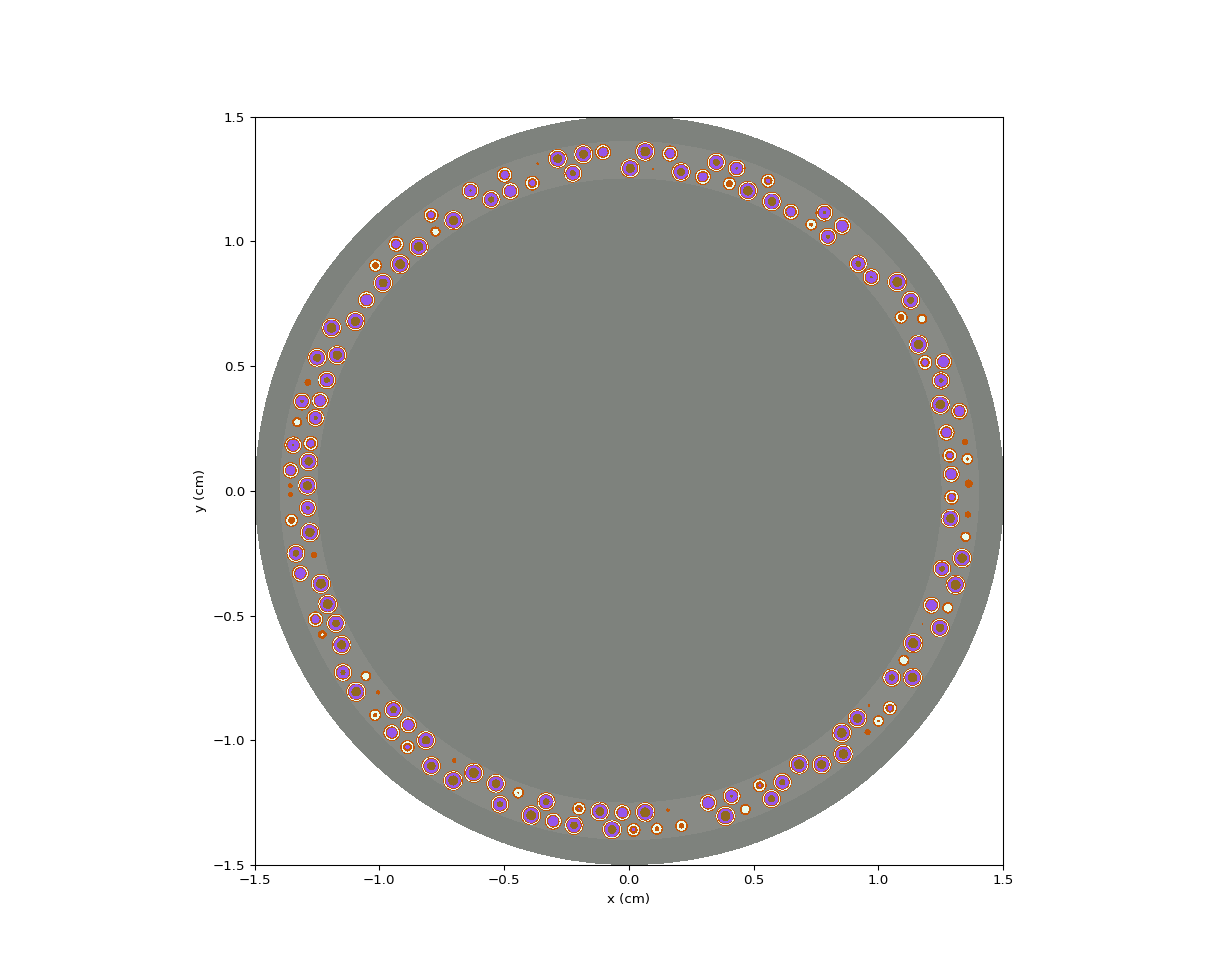
\includegraphics[width=0.5\textwidth]{Figures/pebble_cutaway}}
    \hspace*{.2in}
    \raisebox{-0.5\height}{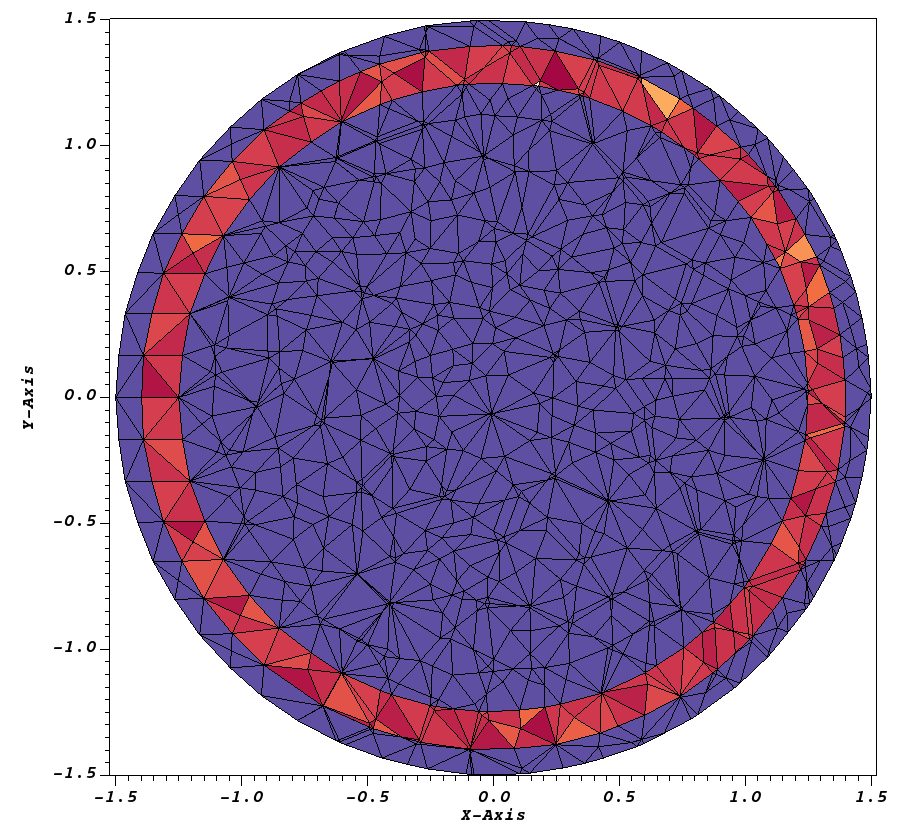
\includegraphics[width=0.365\textwidth]{Figures/umesh_ex}}
    \caption{Qualitative view of a heating tally on an unstructured mesh. Left: Cut-away of the pebble geometry as represented in OpenMC. Right: Result of an applied heating tally where heating occurs only in the region of the pebble containing TRISO particles.}
    \label{fig:pebble_umesh}
\end{figure}

A mesh for each pebble is applied in the Cardinal problem to capture the heat generation distribution throughout the pebble bed. In order to avoid replicating a mesh representing all of the pebbles from either MOOSE or NekRS, the addition of translations to mesh filters was introduced in OpenMC. Placing the translation at this layer of the tally model allows all tallies to rely on a single LibMesh mesh instance acting as a template to represent any pebble in the bed, as shown in \autoref{fig:umesh_tally_steup}. This results in a minimal memory footprint for the tally, even tallying energy deposition for an entire pebble bed.

\begin{figure}[ht]
    \centering
    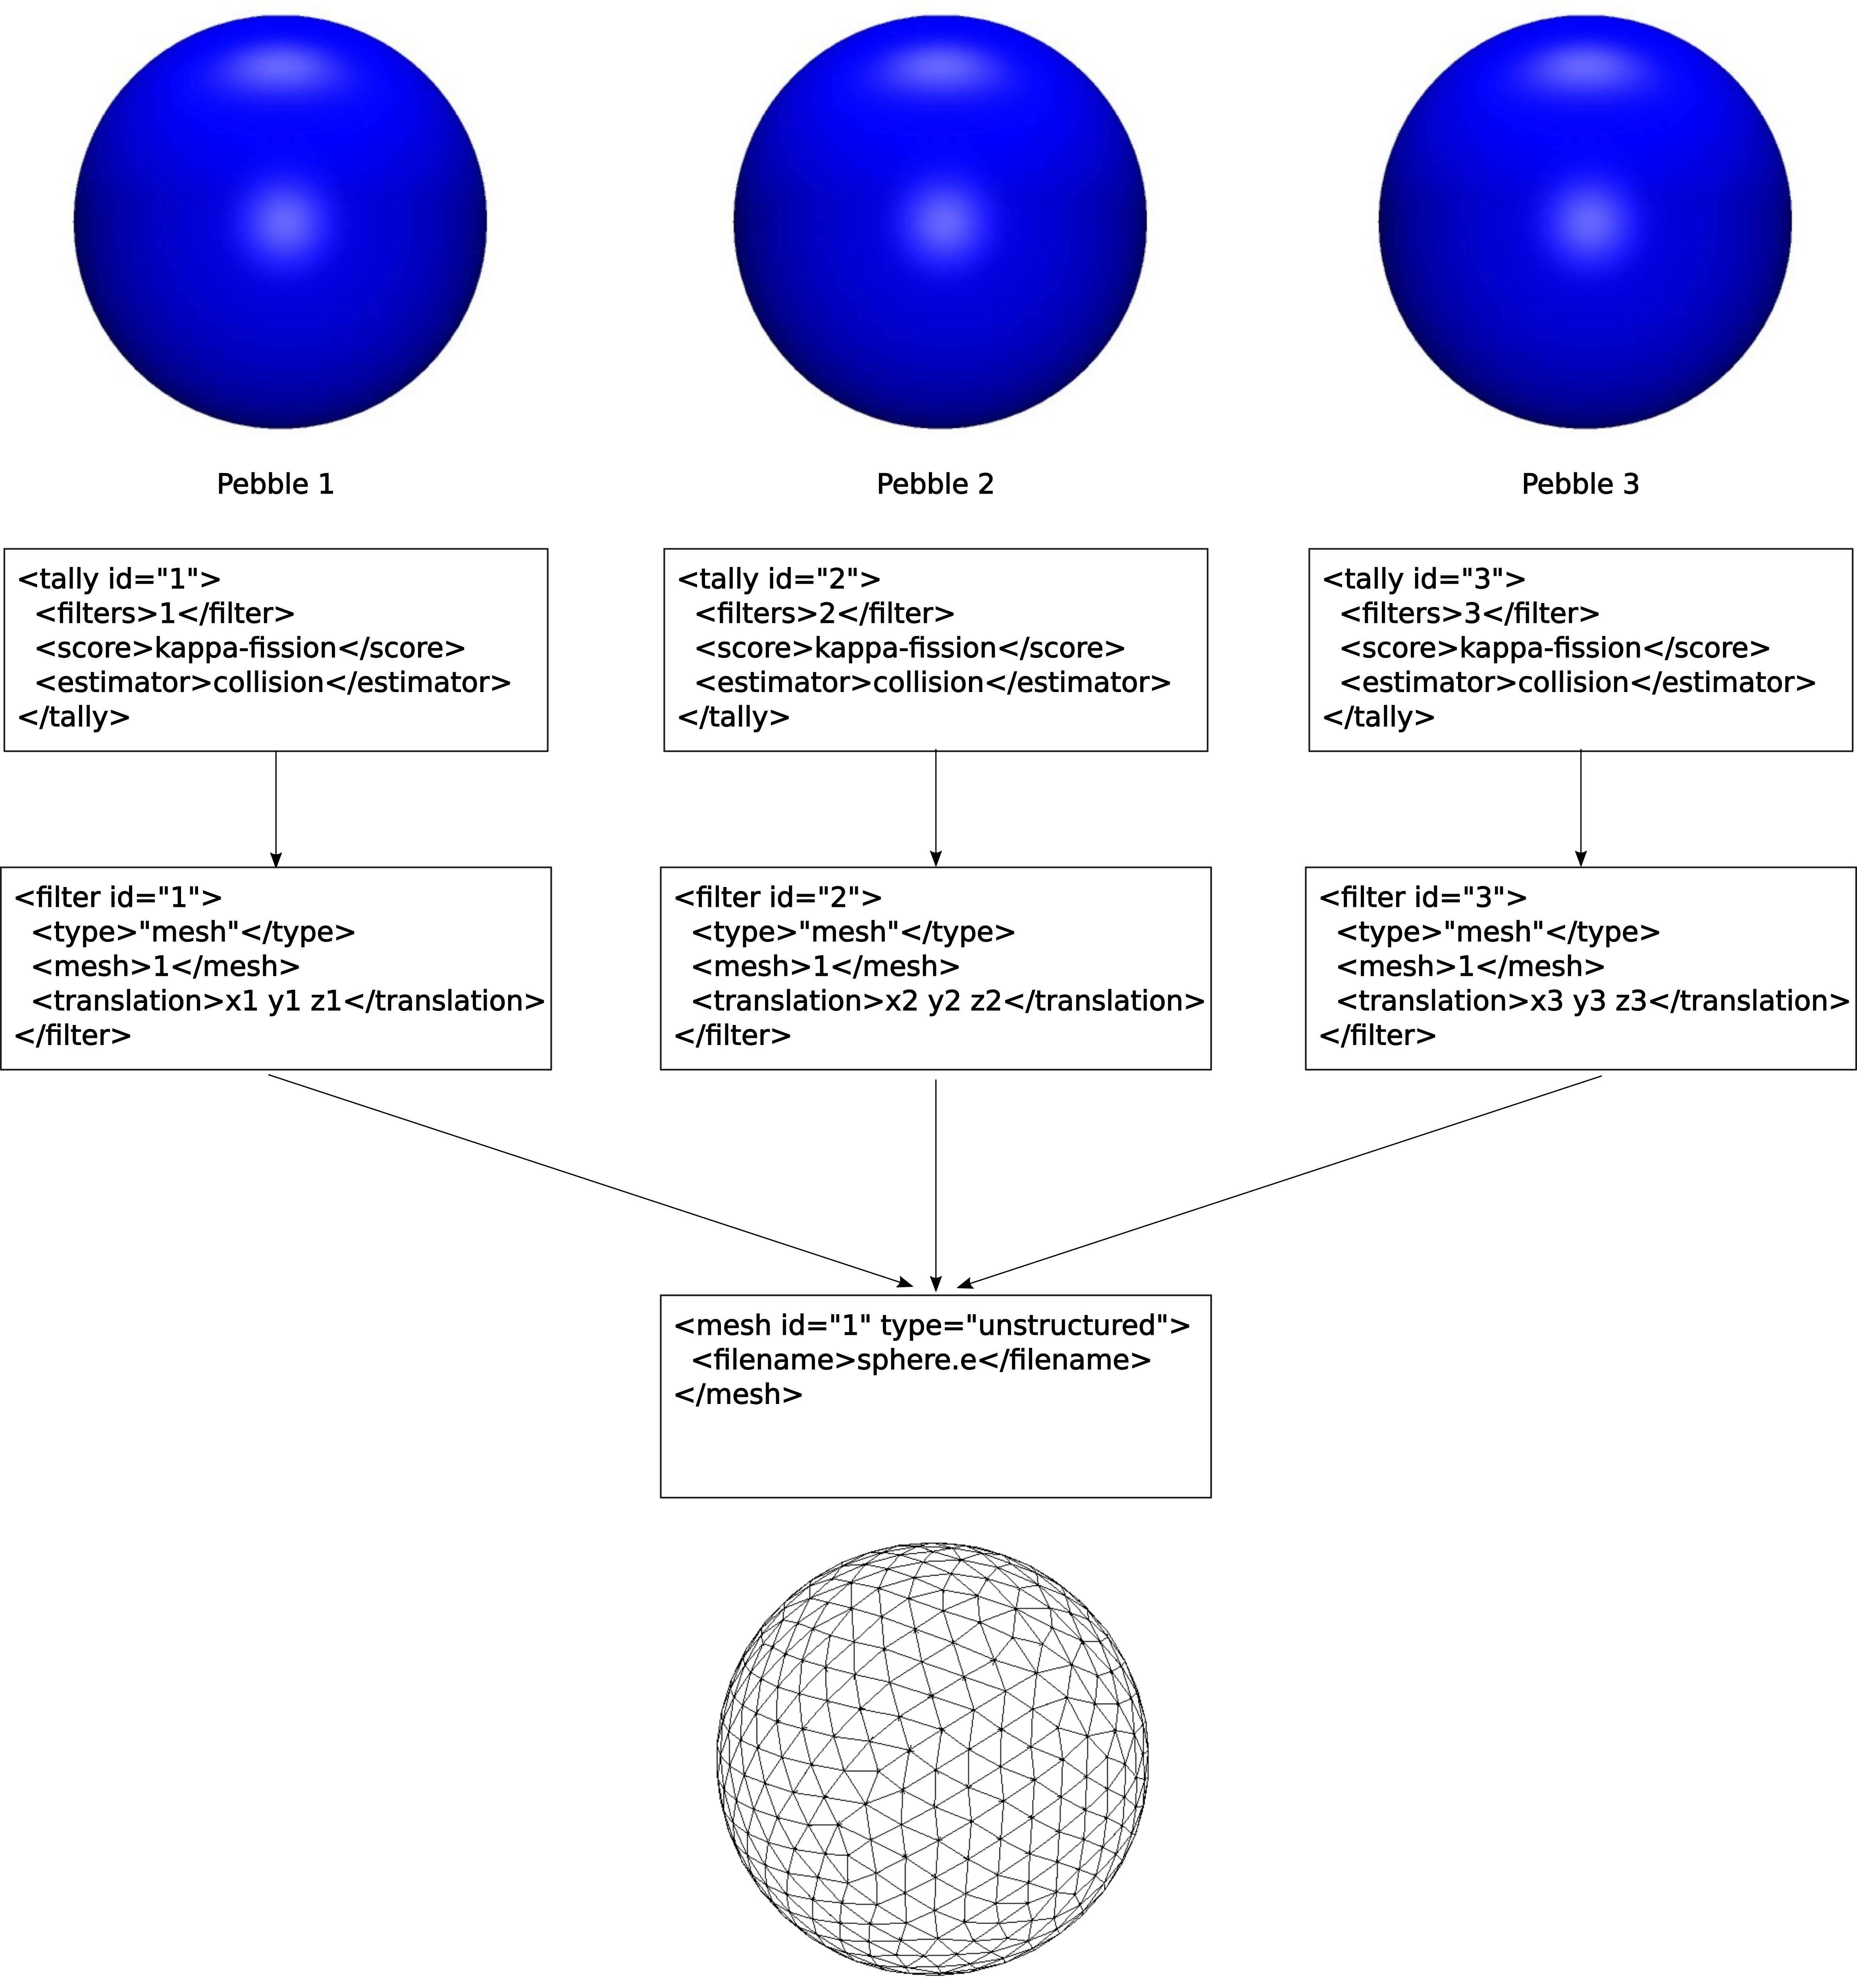
\includegraphics[width=\textwidth]{Figures/umesh_tally_diagram}
    \caption{Organization of unstructured mesh tallies for heat generation in OpenMC.}
    \label{fig:umesh_tally_steup}
\end{figure}

The translation values for each mesh filter are set using the list of pebble centers provided in the MOOSE input file. During problem initialization, these translations are used to calculate the location of element centers in the MOOSE mesh when transferring heat generation values to MOOSE.
% Element volumes can be determined directly from the

Temperature values from MOOSE are updated in OpenMC by using an average temperature value at the pebble center. An option has been added in OpenMC to automatically update the temperature value of all cells inside a pebble to simplify this process.

\subsubsection{BISON}

BISON is a MOOSE-based \cite{hales2013triso, williamson2012multidimensional} nuclear fuel simulation tool developed primarily at Idaho National Laboratory.
BISON is capable of performing high-fidelity finite-element simulation of various fuel forms, including
light-water reactor fuel rods, TRISO fuel particles, and plate fuel. MOOSE allows BISON to solve many
coupled physics, including heat conduction, solid mechanics, burnup, material evolution, plasticity, creep,
fracture, fission gas buildup, gap heat conduction, and neutron embrittlement. In addition, BISON uses
MOOSE to perform these coupled simulations within an implicit solution scheme allowing for long timesteps
and high-order time integration necessary for simulation of operating reactors.

BISON is a high-fidelity tool that has been developed to achieve predictive capability. It has undergone
rigorous assessment testing and verification analysis to ensure accurate simulation. Further, BISON is
developed by using a rigorous V\&V plan. We note that since BISON is a native MOOSE-based application, there is no need for an API. We note also that calculations performed in this manuscript exercise only the conduction module, without any sophisticated fuel performance modeling as an initial demonstration step.
